\section{Design}

Our design is split up in three modules.
\begin{description}
    \item[bohnanza] {Mostly an abstract base module that contains logic for both the std and
    hb game.}
    \item[bohnanza-std] {A concrete module that uses the \emph{bohnanza} module in order to play
    the std bohnanza game.}
    \item[bohnanza-hb] {A concrete module that uses the \emph{bohnanza} module in order to play the
    hb bohnanza game.}
\end{description}
The reason why these elements are composed this way and called modules is a result of the dependency
injection (Guice\footnote{https://code.google.com/p/google-guice/}) framework we use. This framework supplies abstract module classes which
need to be implemented. Such a module class contains a set of dependencies. For example the bohnanza module uses an abstract Player class.
Both the bohnanza- and bohnanza-hb module use an concrete implementation hereof. Another reason why these modules are composed this way
is due to the fact that we chose an extension (and the std game) should extend classes of the base game and not implement hooks. 

Every module is designed according to the MVC pattern. The main classes that are involved in the MVC pattern are shown in Figure
\ref{fig:design:mvc}.

 \begin{figure}[h!]
    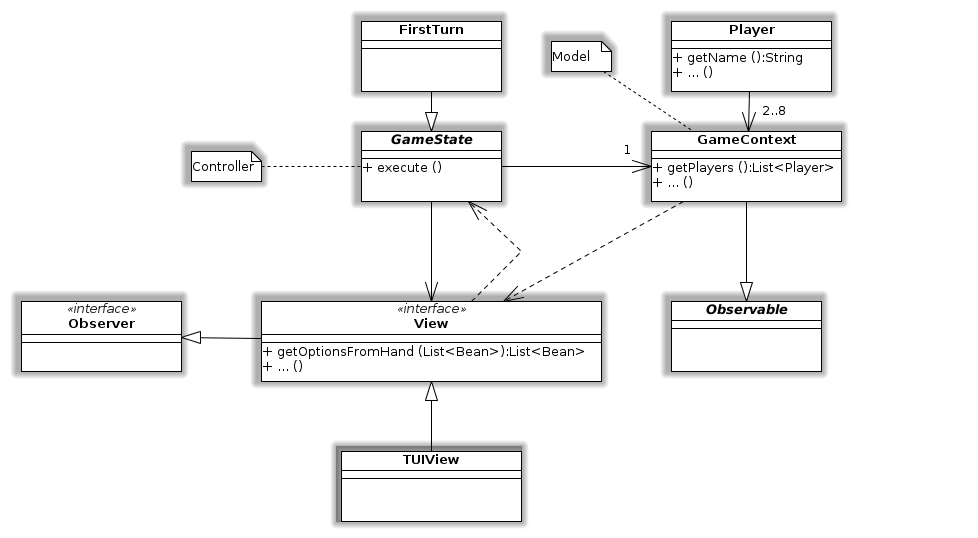
\includegraphics[width=\textwidth]{../img/Mvc}
    \caption{Classes involved in MVC} 
    \label{fig:design:mvc}
\end{figure}

The \texttt{GameContext} is the main model class. It contains many assocations to other model classes such as the \texttt{Player}. Many
model classes are \texttt{Observable} by \texttt{Observer}s such as the \texttt{View} class; this is how the view knows the status of the
model. We could also have given the \texttt{GameContext} to the \texttt{View}.

The \texttt{GameState} is the controller which updates the view and the model and is part of a \emph{state} pattern. The controller issues
method calls such as \texttt{getOptionsFromHand()} in the view and the method returns a sub set of \texttt{Bean} cards. An alternative to
the MVC pattern is the Model View Presenter pattern which could have been applied in this context. We chose to keep things simple and focus more on the
extensibility of bohnanza rather than on implementing other views such as a graphical one. We think that the classic MVC pattern suffices
here. 
 
\subsection{Model}
Three important parts of the model involve the hierarchy of cards (Figure \ref{fig:design:cards}),
the creation of cards (Figure \ref{fig:design:creator}) using a \emph{factory method} pattern and
the relation between different sets of cards and the players (Figure \ref{fig:design:player}). 

 \begin{figure}[h!]
    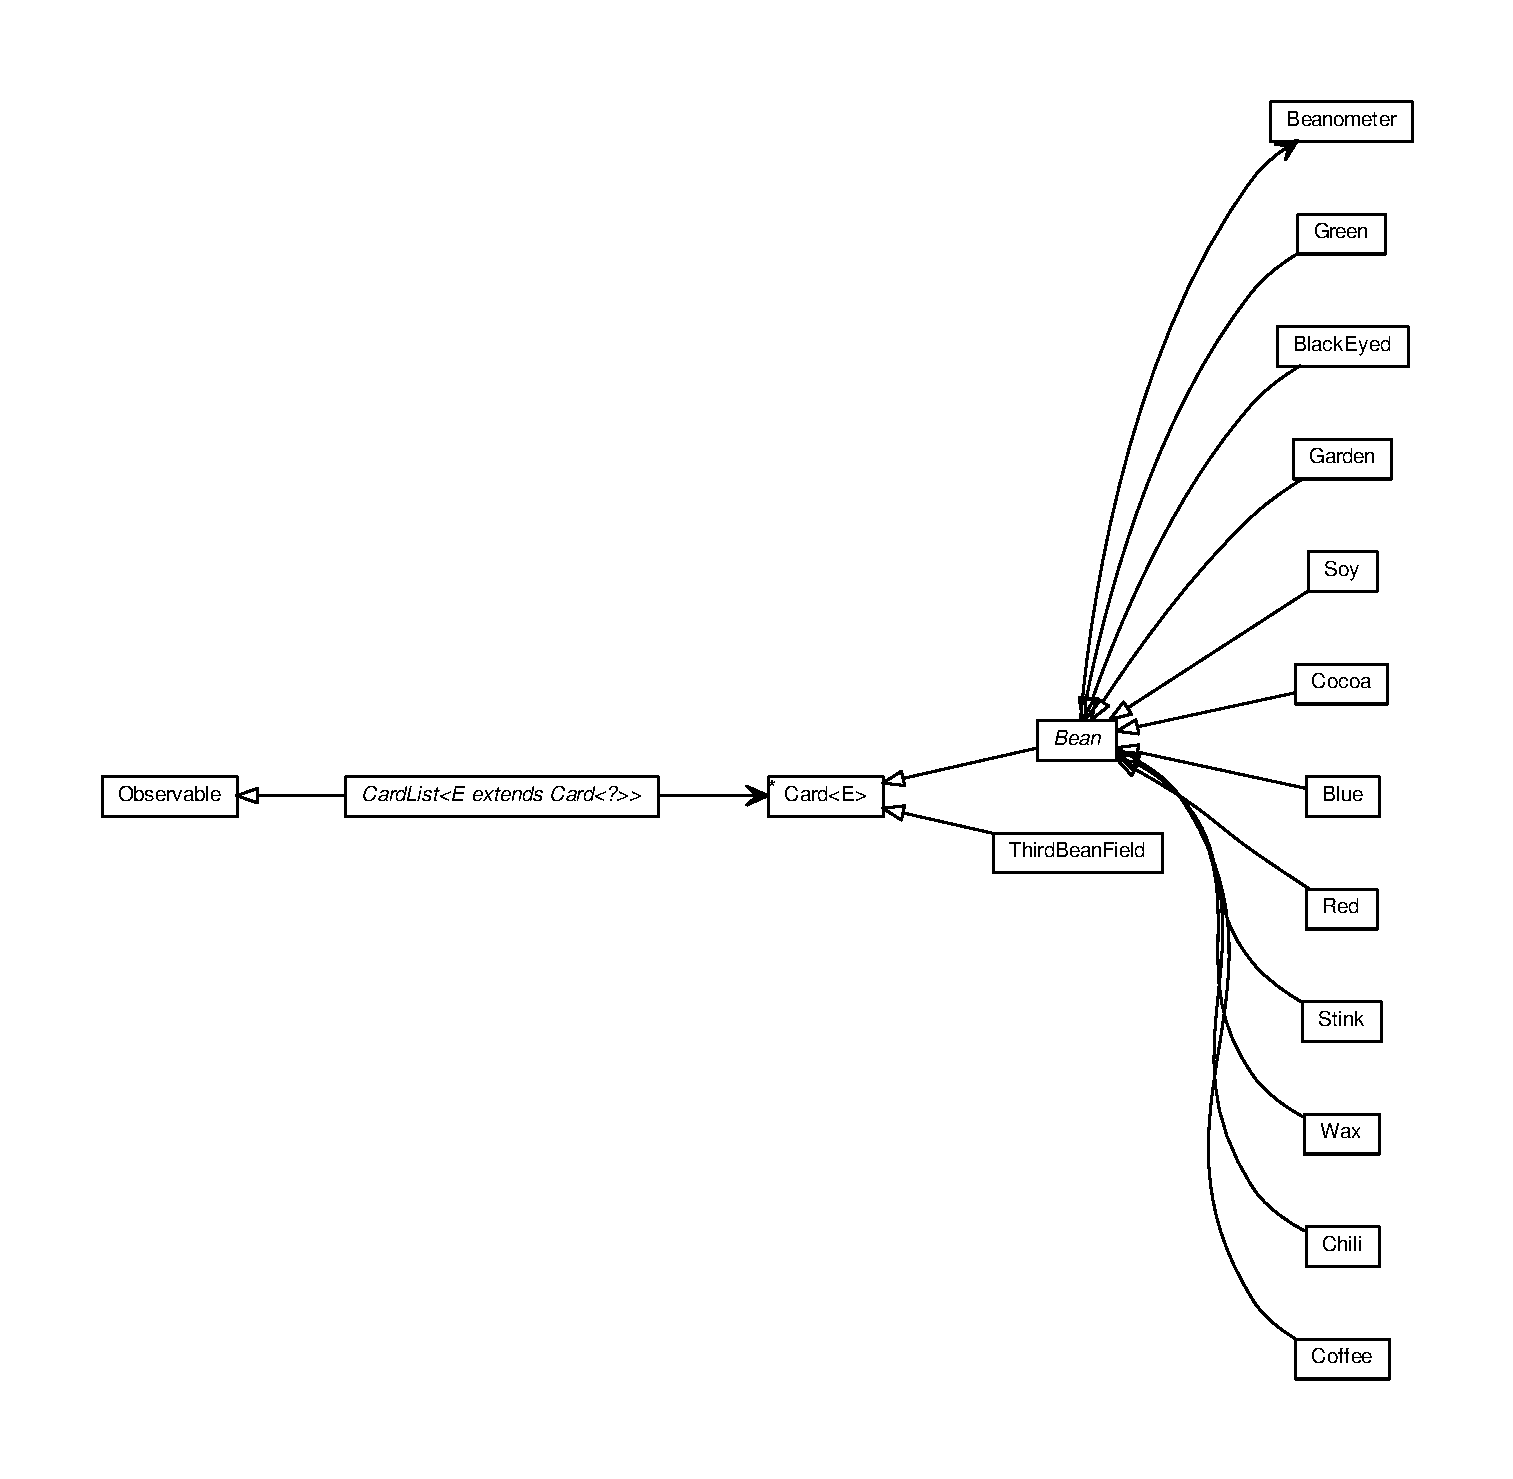
\includegraphics[width=\textwidth]{../umlgraph/CardGraph}
    \caption{Class diagram of the cards}
    \label{fig:design:cards}
\end{figure}

\begin{figure}[h!]
    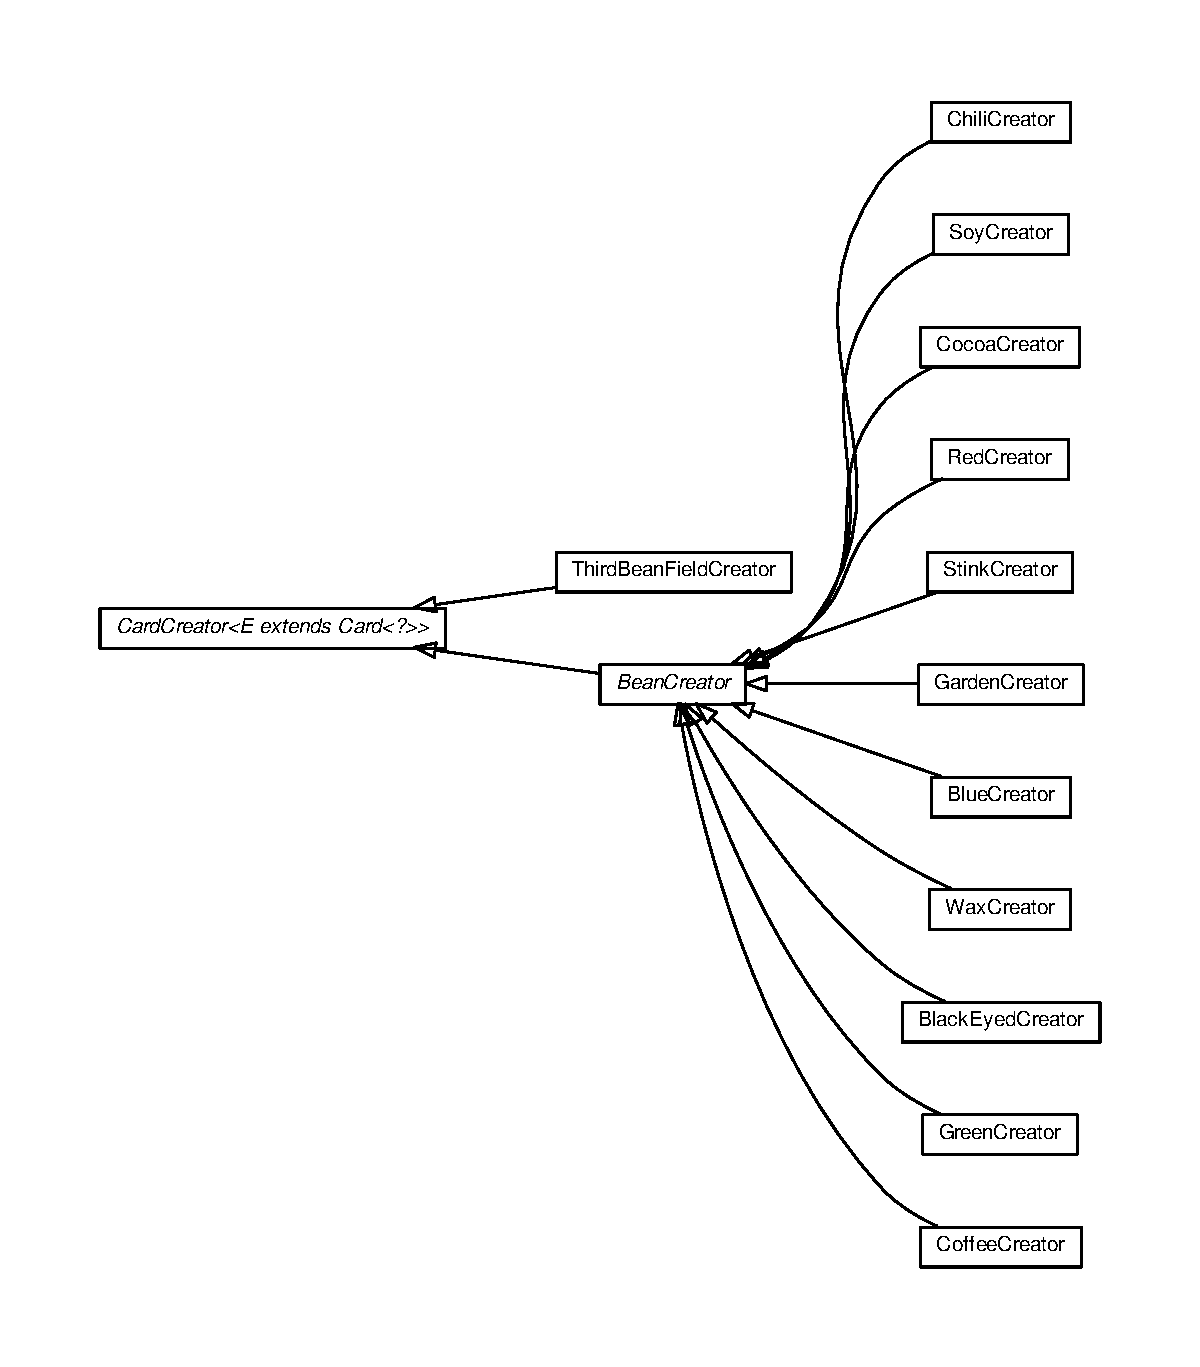
\includegraphics[width=\textwidth]{../umlgraph/CreatorGraph}
    \caption{Class diagram for the creation of cards}
    \label{fig:design:creator}
\end{figure}

The hierarchy of the cards here is convenient, namely when creating extensions of bohnanza. When new cards are introduced to the game
creating a new factory i.e. subtyping \texttt{CardCreator} or \texttt{BeanCreator} is easy because those factories expect to create a
subtype of a \texttt{Card}. Instead of using a factory method pattern we could have approached this a little different. Guice allows
creating multiple instances of a class by means of a \texttt{Provider} class. Using this alternative would have resulted in cleaner code. The reason why we
did not choose this alternative is because we introduced Guice into our project after we used the factory method pattern and did not want to
restructure our code. We did however use the provider method for creating \texttt{Player}s as shown in Figure \ref{fig:design:di}, because
this was the only way to inject these objects into an \texttt{Bohnanza} object.
 
\begin{figure}[h!] 
    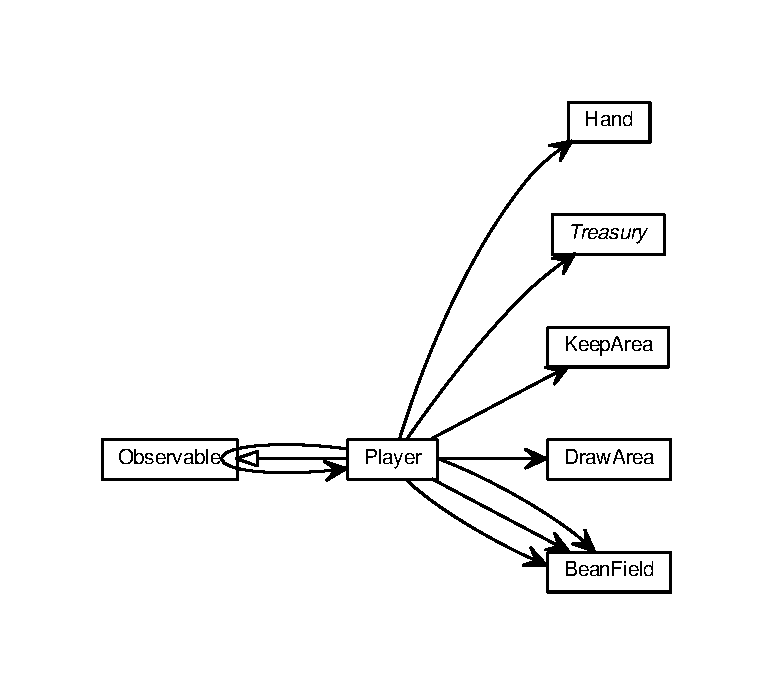
\includegraphics[width=\textwidth]{../umlgraph/PlayerGraph}
    \caption{Class diagram for the player and association to particular sets of cards}
    \label{fig:design:player}
\end{figure}

\newpage
\subsection{Controller}
The controller of the game is implemented using a \emph{state} design pattern and is shown in Figure
\ref{fig:design:controller}. In bohnanza the order of states is rather fixed, the order
only varies depending on how often the deck is shuffled or in case of execeptional behaviour. In case exceptional behaviour occurs in our application the next state is always the
\texttt{Fail} state. In general the order of states that are executed are \texttt{Prepare} \textrightarrow{} \texttt{FirstTurn}
\textrightarrow{} \texttt{SecondTurn} \textrightarrow{} \texttt{ThirdTurn} \textrightarrow{} \texttt{FourthTurn} \textrightarrow{}
\texttt{FirstTurn} \textrightarrow{} \ldots \textrightarrow{} \texttt{End}. A typical implementation of the \texttt{GameState.execute}
method is shown from \texttt{FirstTurn} in Listing \ref{lst:firstturn-execute}. Note how the next state is set by getting the singleton
instance on Line 19.
The application continues until a \texttt{GameState} sets the next state to \texttt{null}, i.e. when \texttt{GameContext.getState() == null}.

\begin{lstlisting}[language=Java, caption=FirstTurn.execute(), label=lst:firstturn-execute]
@Override
public void execute(GameContext context) {

    if (context.getCurrentPlayer().getHand().size() > 0) {

        int beanFieldNumber = context.getView().mustPlant(context.getCurrentPlayer());

        try {

            context.getCurrentPlayer().plantHand(beanFieldNumber);
 
            if (context.getCurrentPlayer().getHand().size() > 0) {
                beanFieldNumber = context.getView().mayPlant(context.getCurrentPlayer());

                context.getCurrentPlayer().plantHand(beanFieldNumber);

            }

            context.changeState(SecondTurn.getInstance());

        } catch (BohnanzaException e) {
            context.changeState(Fail.getInstance());
            Fail.getInstance().setException(e);
        }
    }
}
\end{lstlisting}

As concrete state classes we could have merged states such as the first turn and second turn. But we split the states the way we did,
because they form units which can conveniently be tested in isolation. An entirely alternative design pattern for the controller we could
use here is the \emph{strategy} pattern. The strategy pattern is more applicable in situations where strategies are chosen at runtime. But more importantly
the strategy pattern is used in situations where the result of different strategies is the same, of course in bohnanza this is not the case. 

\begin{figure}[h!]
    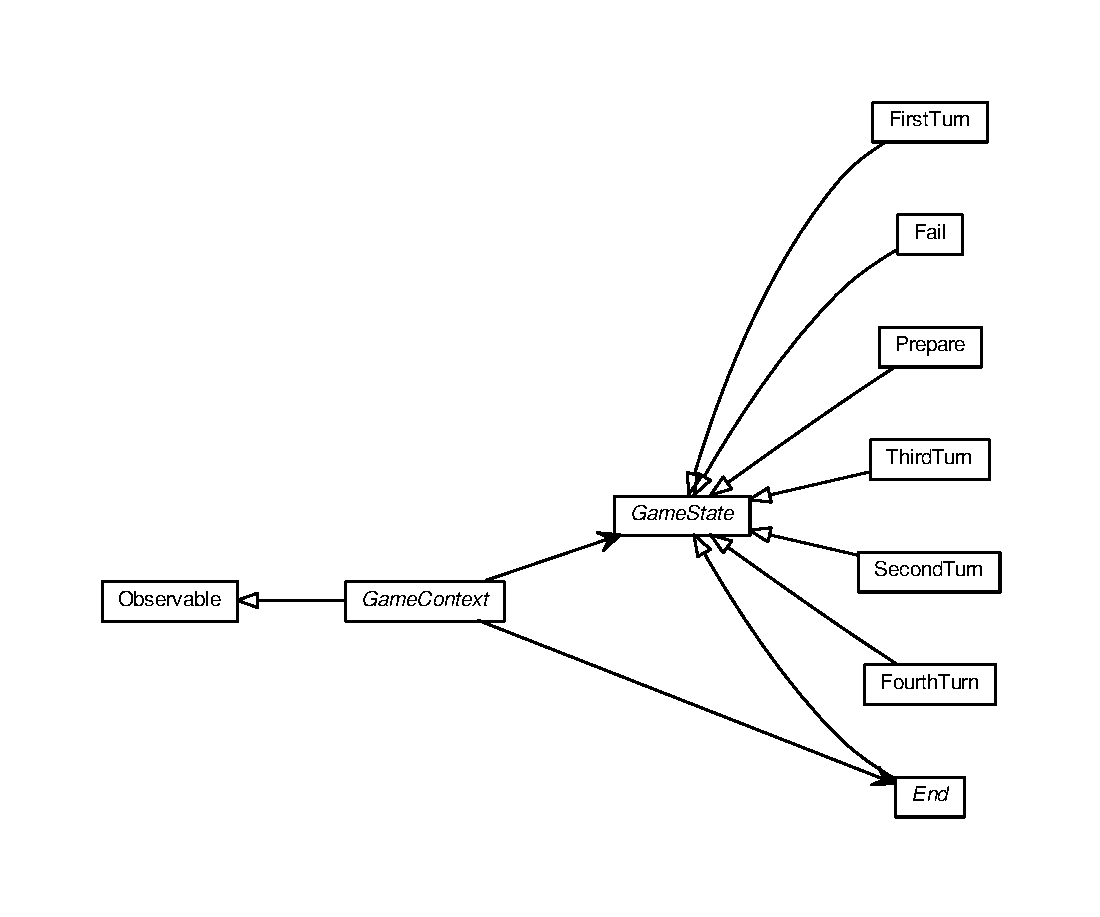
\includegraphics[width=\textwidth]{../umlgraph/StateGraph}
    \caption{Class diagram for controlling the state of the game}
    \label{fig:design:controller}
\end{figure}

\subsection{View}
Currently we support only a textual user interface. The \texttt{TUIView} class is an implementation
of a \texttt{View} interface. Creating a new interface like a graphical or a network would involve
implementing the \texttt{View} interface.

\subsection{Packages}
Our modules contain the following packages.
\begin{description}
\item[bohnanza] contains the main class.
\item[bohnanza.game] contain some models for bohnanza, such as a \texttt{Card}.
\item[bohnanza.game.factory] contains classes w.r.t. the creation of cards.
\item[bohnanza.game.player] contains model classes w.r.t. the player.
\item[bohnanza.game.shared] contains model classes which may be accessed by all players.
\item[bohnanza.game.gameplay] contains controller classes w.r.t. the discussed state pattern.
\item[bohnanza.module] contains classes w.r.t. dependency injection of Guice.
\item[bohnanza.umlgraph] contains classes that model UML graphs used in this report.
\item[bohnanza.view] contains the view classes.
\end{description}

The packages are rather self explanatory. It can be argued however that some packages such as \texttt{bohnanza.game.player} and
\texttt{bohnanza.game.shared} may be merged. We did not do this because in an early stage of the development we chose to make some classes
\emph{package private} such that for example only a \texttt{Player} could construct a \texttt{Hand}. This would make sure there can only be as many \texttt{Hand}s in
the game as there are \texttt{Player}s. This design choice was one of the reasons our code was not testable and we had to change the visibility
parameters to use dependency injection.

\subsection{Variations}

\subsubsection{User}
The user can specify during the start up of the application how many players there are using a
command line option. For example \texttt{java bohnanza.BohnanzaStd -p=3} starts the BohnanzaStd
module with three players. Parsing command line options is done using the Apache Commons CLI library.

\subsubsection{Developer}
Variability for the developer depends heavily on notion of \emph{dependency injection}. Dependency
injection is a design pattern that basically involves moving dependency resolution from a particular
class to a framework dedicated to dependency injection. Classes involved with dependency injection are shown in
Figure \ref{fig:design:di}. If a developer wants another variation of the application the developer can simply extend the
\texttt{BohnanzaModule} class and define other classes to inject, note that BohnanzaModule
extends the \texttt{AbstractModule} class from Guice. For example if a \texttt{Hand} object needs
to behave differently for a particular extension of bohnanza one can extend the \texttt{Hand} class and
define the extension in the extension of BohnanzaModule. 

BohnanzaModule itself is
an abstract class and this class only knows the full list of required dependencies. A concrete class
such as BohnanzaStdModule implements some methods that return concrete classes as
dependencies. This relates closely to the \emph{single choice principle}. Listing \ref{lst:di} shows how one can change dependencies using
an extension of the AbstractModule class. Note how the singleton pattern and the provider incorporate nicely in the configure method.

\begin{lstlisting}[language=Java, caption=BohnanzaModule.java, label=lst:di]
public abstract class BohnanzaModule extends AbstractModule {

    @Override
    protected void configure() {
        bind(View.class).to(getViewClass());
        bind(DrawDeck.class).in(Singleton.class);
        bind(Player.class).toProvider(getPlayerProviderClass());
        ...
    }

    protected abstract Class<? extends Provider<? extends Player>> getPlayerProviderClass();
    protected abstract Class<? extends DrawDeck> getDrawDeckClass();
    protected abstract Class<? extends View> getViewClass();    
    ...
}
\end{lstlisting}

We have not really considered an alternative to dependency injection, because to our knowledge there is no real alternative
for it. There is however the service locater pattern, but both these patterns solve a problem which
is not that hard, that is injecting instances of some classes in another object instead of
constructing these instances in that particular object. We found that Guice was a good enough
framework, so we did not consider an alternate framework. 

\begin{figure}[h!]
    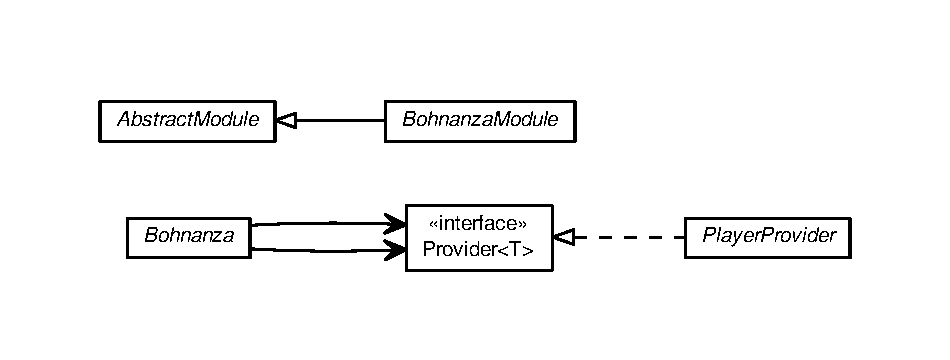
\includegraphics[width=\textwidth]{../umlgraph/ModuleGraph}
    \caption{Class diagram of classes involving dependency injection}
    \label{fig:design:di}
\end{figure}
